\header{7}
\chapter{Krachten op het schip}
\section{Inleiding}
In voorbereiding op het leren van een aantal zeilmanoeuvres is het belangrijk om de krachten op het schip goed te snappen. In dit hoofdstuk gaan we onder andere kijken naar hoe krachten weergegeven kunnen worden en de verschillende effecten van deze krachten. 
\section{Krachten weergeven}
Een kracht wordt weergegeven met een pijl. De richting van de pijl geeft de richting van de kracht weer en de lengte geeft de grootte van de kracht weer. In figuur \ref{pic:kracht} is een voorbeeld te zien.

De wind wordt meestal met één pijl aangegeven. In werkelijkheid komt de wind meer als een vlak op je af. Het zijn als het ware heel veel pijlen met dezelfde richting naast elkaar. Dit is te zien in figuur \ref{pic:wind_pijl}.

Tot slot is er nog het draaipunt. Wanneer er een kracht op een voorwerp met draaipunt gezet wordt, draait deze om het draaipunt. Bij een boot zit het draaipunt ongeveer bij de mast. In figuur \ref{pic:draaipunt} is hier een voorbeeld van gegeven. Je zou de tekening een beetje met een wip kunnen vergelijken.
\begin{figure}[h]
  \centering
  \begin{minipage}[b]{0.32\textwidth}
  \centering
    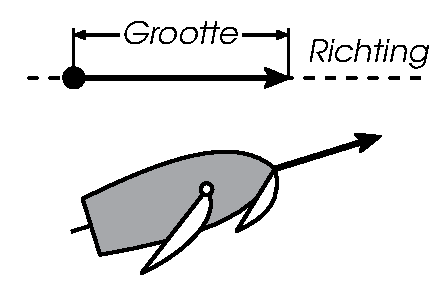
\includegraphics[width=0.8\textwidth]{../Hoofdstukken/Krachten/pdf/krachten.pdf}
    \caption{Krachten}
    \label{pic:kracht}
  \end{minipage}
  \hfill
  \begin{minipage}[b]{0.32\textwidth}
    \centering
    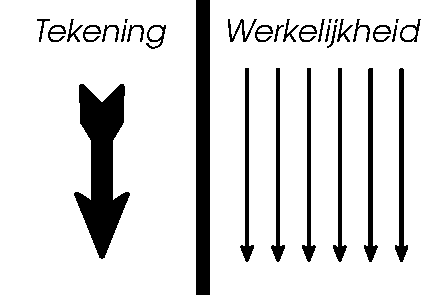
\includegraphics[width=0.8\textwidth]{Hoofdstukken/Krachten/pdf/wind.pdf}
    \caption{Wind pijlen}
    \label{pic:wind_pijl}
    \end{minipage}
  \hfill
  \begin{minipage}[b]{0.32\textwidth}
    \centering
    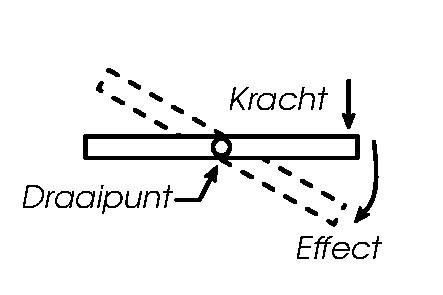
\includegraphics[width=0.8\textwidth]{Hoofdstukken/Krachten/pdf/draaipunt.pdf}
    \caption{Draaipunt}
    \label{pic:draaipunt}
  \end{minipage}
\end{figure}
\section{Effecten van de fok en het grootzeil}
Het grootzeil en de fok hebben allebei een ander effect op de boot. Omdat de fok voor het draaipunt zit, zorgt deze voor afvallen. Dit is te zien in figuur \ref{pic:effect_fok}.

Het grootzeil doet het tegenovergestelde omdat deze achter het draaipunt zit. Hierdoor zal de boot gaan oploeven. Dit effect is weergegeven in figuur \ref{pic:effect_grootzeil}.
\begin{figure}[ht]
  \centering
  \begin{minipage}[b]{0.49\textwidth}
  \centering
    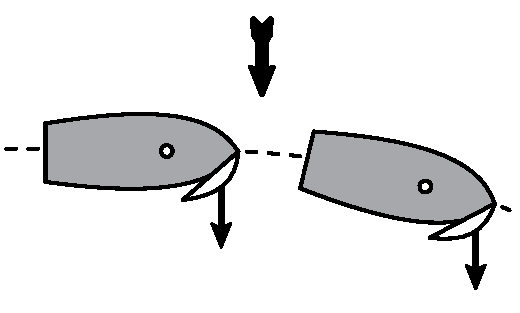
\includegraphics[width=0.8\textwidth]{../Hoofdstukken/Krachten/pdf/effect_fok.pdf}
    \caption{Effect van de fok}
    \label{pic:effect_fok}
  \end{minipage}
  \hfill
  \begin{minipage}[b]{0.49\textwidth}
    \centering
    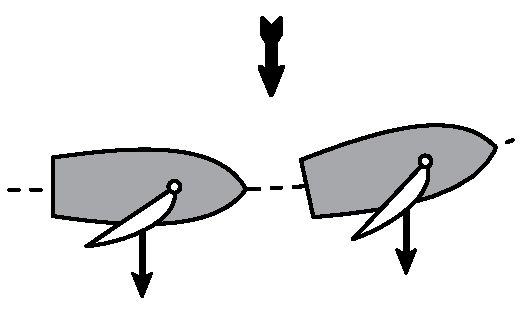
\includegraphics[width=0.8\textwidth]{../Hoofdstukken/Krachten/pdf/effect_grootzeil.pdf}
    \caption{Effect van het grootzeil}
    \label{pic:effect_grootzeil}
    \end{minipage}
\end{figure}
\section{Correcte zeilstand}
We beginnen door te kijken naar wanneer het grootzeil goed staat. Een voorbeeld van een zeil wat goed staat is te zien in figuur \ref{pic:zeil_goed}. De windpijlen stormen mooi, dicht langs het zeil. Het zeil vervormt niet door de wind en staat mooi bol.

Wanneer je het zeil echter te strak aan trekt, zie je in figuur \ref{pic:zeil_strak} dat de wind pijlen aan de buitenkant van het zeil "loslaten". De wind wil liever rechtdoor dan dicht langs het zeil. Hierdoor ontstaan er in dit stukje wervelingen. Door deze wervelingen gaat het achterlijk van je zeil klapperen. Je zeil staat niet meer goed en hierdoor ga je langzamer zeilen.    
\begin{figure}[H]
  \centering
  \begin{minipage}[b]{0.32\textwidth}
  \centering
    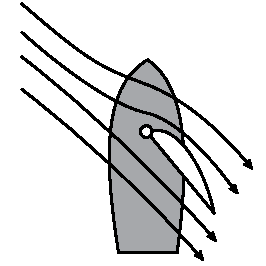
\includegraphics[width=0.85\textwidth]{Hoofdstukken/Krachten/pdf/zeil_goed.pdf}
    \caption{Zeil goed}
    \label{pic:zeil_goed}
  \end{minipage}
  \hfill
  \begin{minipage}[b]{0.32\textwidth}
    \centering
    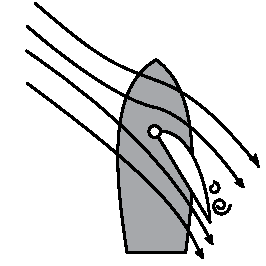
\includegraphics[width=0.85\textwidth]{../Hoofdstukken/Krachten/pdf/zeil_strak.pdf}
    \caption{Zeil te strak}
    \label{pic:zeil_strak}
    \end{minipage}
  \hfill
  \begin{minipage}[b]{0.32\textwidth}
    \centering
    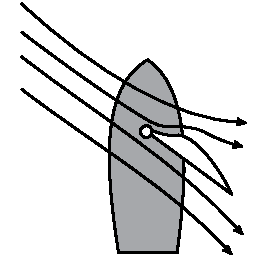
\includegraphics[width=0.85\textwidth]{Hoofdstukken/Krachten/pdf/zeil_los.pdf}
    \caption{Zeil te los}
    \label{pic:zeil_los}
  \end{minipage}
\end{figure}
Een andere manier waar op je zeil verkeerd kan staan is als hij te los is. Dit is afgebeeld in figuur \ref{pic:zeil_los}. Het zeil zit nu als het ware in de weg van de wind. De windpijlen botsen bij het voorlijk van je zeil met het zeil. Hierdoor ontstaat er een tegen bolling dicht bij je mast. Dit remt je ook af. 

Een goede manier om je zeil te stellen, is om hem net zo lang te laten vieren, totdat je een kleine tegenbolling ziet in het voorlijk. Dan trek je het zeil weer een klein beetje aan. Op deze manier benut je de wind maximaal. Door dit regelmatig te doen weet je zeker dat je optimaal zeilt. 
\section{Effect van de helling}
De helling van je boot (oftewel, hoe schuin je vaart) heeft ook effect op het gedrag van de boot. Met name op de loef- en lijgierigheid. Uit zichzelf is de boot loefgierig. Dit houdt in dat de boot vanzelf de wind in draait als er niets gebeurt. 

Door de boot te laten hellen naar de lijkant, kan je dit effect versterken. Hoe meer mensen er bijvoorbeeld aan de lijkant in de boot zitten, hoe sneller de boot oploeft. Het tegenovergestelde geldt voor de loefkant. Als je naar deze kant helt, wil de boot uit zichzelf afvallen. 
\section{Conclusie}
In dit hoofdstuk zijn de verschillende krachten op het schip behandeld. Je snapt nu wanneer een zeil goed en fout staat en hoe je je zeil makkelijk goed kan zetten. Daarnaast snap je welke krachten er op het schip zijn, wat ze doen en hoe je deze in je voordeel kunt gebruiken.  